\documentclass[]{standalone}
\usepackage{pgfplots}
\usepackage{pgfplotstable}
\usepgfplotslibrary{polar}
\pgfplotsset{compat=1.16}

\begin{document}
\begin{tikzpicture}
    \begin{polaraxis}[
        xtick={0,45,...,315},
        ytick=\empty,
        colormap/viridis,
    ]
    \addplot [point meta=y, scatter, only marks, draw opacity=0]
        table [x=direction, y=0.45, col sep=comma] {test.csv};
    \end{polaraxis}
\end{tikzpicture}

\begin{tikzpicture}[%
]
\begin{axis}[%
point meta min=0,
point meta max=360,
y dir=reverse,
hide axis,
]
\addplot [] graphics [xmin=0.5,xmax=360.5,ymin=0.5,ymax=360.5]
{dev/test.png};
\end{axis}
\end{tikzpicture}%

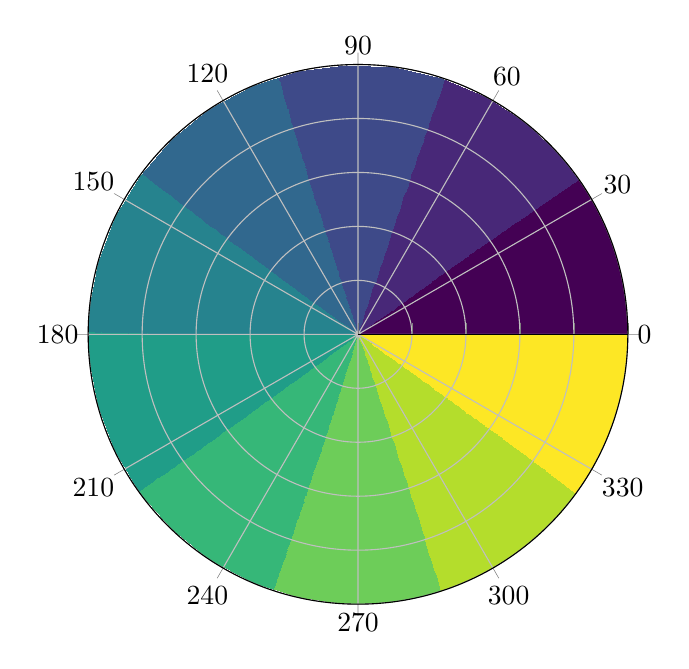
\begin{tikzpicture}
\begin{polaraxis}[
yticklabels = {},
ymin=0, ymax=1,
colormap name={viridis},
axis on top=true,
]
\addplot3[contour filled={number=10},
        samples=36, domain=0:360, y domain=0:1,
    ]
    {+x+y};
\end{polaraxis}
\end{tikzpicture}

\begin{tikzpicture}
\begin{polaraxis}[
    xtick={0,45,...,315},
    ytick=\empty,
    colormap/viridis,
    tickwidth=0,
    xtick distance = 45,
    % separate axis lines,
    y axis line style= { draw opacity=0 },
    ymin=0, ymax=90,
    axis on top=true,
]
\addplot3 [surf] file {dev/ohist.dat};
\end{polaraxis}
\end{tikzpicture}

\end{document}